\documentclass[a4paper, 12pt]{article}

%\usepackage[margin = 3cm]{geometry}
\usepackage[normalem]{ulem}
\usepackage[french]{babel}
\usepackage[utf8]{inputenc}
\usepackage[T1]{fontenc}
\usepackage{graphicx}
\usepackage{hyperref}
\usepackage{enumitem}
\usepackage{fancyhdr}
\usepackage{fullpage}
\usepackage{xcolor}
\usepackage{setspace}
\usepackage{amsmath}
\usepackage{calc}
\usepackage{relsize} 
\usepackage{times}
\usepackage{amssymb}
\usepackage[ruled,vlined]{algorithm2e}
\usepackage{enumitem}
\usepackage{fullpage}
\usepackage{xcolor}
\usepackage{setspace}
\usepackage{calc}
\usepackage{relsize}
\usepackage{tikz}

\graphicspath{ {./images/} }

\usepackage[bottom]{footmisc}

%\setlength{\headheight}{22.6pt}
\setlength{\parskip}{1em}
\renewcommand{\baselinestretch}{1.1}

\include{pythonlisting}


\title{
    {\bf FMSI}
}
\author{
    { \bf --- Auteurs: --- }
    \\ Alexandre Dias
    \\ Bastien Coutadeur
    \\ Benjamin Peter
    \\ Mathieu Guérin
}
\date{24 avril 2021}

\pagestyle{fancy}

\fancyhead{} % clear all header fields
\renewcommand{\headrulewidth}{0pt} % no line in header area
\fancyfoot{} % clear all footer fields
\renewcommand{\footrulewidth}{1pt} % line in footer area

\lfoot{FMSI}
\cfoot{}
\rfoot{\thepage}

\begin{document}

\maketitle

\tableofcontents


\newpage
% ---
\section{Introduction}

Afin d'appliquer les différents algorithmes vus en cours, nous nous sommes intéressés aux a leur implémentation ainsi que leur efficacité en fonction de la taille de la clé.
Pour maintenir un temps raisonnable dans les démonstrations, nous nous sommes focalisés sur des nombres 
premiers assez petits par rapport à ce qui est employé dans l'industrie.

Vous pourrez trouver toutes les démonstrations dans le Notebook associé à ce document, il nécessite la bibliothèque Matplotlib afin d'afficher les différents graphes.

Nous ferons dans un premier temps une brève présentation des algorithmes utilisés pour générer les nombres premiers puis, l'algorithme de chiffrement RSA et finalement nous nous pencherons sur les algorithmes Rho-Pollard, p - 1 Pollard et la factorisation de Fermat.

Nous conclurons par une comparaison de ces trois algorithmes implémentés en Python.

Le code source de notre travail est disponible \underline{\href{https://github.com/Unicuby/FMSI/}{ici}}\footnote{https://github.com/Unicuby/FMSI/}.


\newpage
% ---
\section{Génération des nombres premiers}
\subsection{Érathosthène}

Afin de générer des clés RSA nous avons besoin d'utiliser des nombres premiers.

Génération de nombres premiers: \\
Via le crible d'Ératosthène qui consiste à écrire tous les nombres d'un intervalle donné, puis à supprimer les multiples des nombres premiers déjà trouvé, en s'arrêtant à la racine carrée de la borne supérieure de l'intervalle. Les nombres restants sont les nombres premiers de l'intervalle.

\begin{center}
    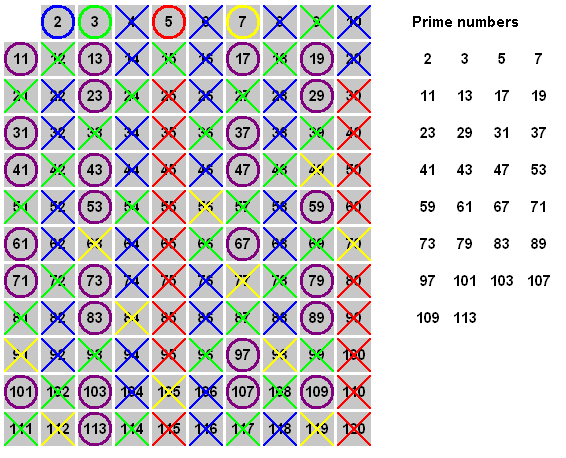
\includegraphics[width=0.8\linewidth]{eratosthene.png}
\end{center}

\newpage
\subsection{Miller-Rabin}

Miller-Rabin est un algorithme de primalité probabiliste, il permet en un temps cours de vérifier si le 
nombre donné est composite mais n'assure pas de manière certaine que le nombre donné est premier.
Un grand nombre d'entiers aléatoires sont générés.

L'algorithme est le suivant:

\begin{algorithm}[H]
\SetAlgoLined
Paramètre 1: $n$ nombre impair \\
Paramètre 2: $limit$ nombre d'entiers utilisés pour tester la primalité de n \\
\KwResult{Vrai s'il n'est pas composite, Faux sinon}
    $s \xleftarrow{} 0$ \;
    $d \xleftarrow{} p - 1$ \;
    \While{$d$ is even}{
        $s \xleftarrow{} s + 1$ \;
        $d \xleftarrow{} d / 2$ \;
    }
    \For{$i = 0$ to $limit$}{
        $a \xleftarrow{} random(2, p - 1)$ \;
        $x \xleftarrow{} a^d[p]$ \;
        
        \If{$x = 1$ ou $x = p - 1$}{
            continue \;
        }
        
        \For{$r$ de $0$ a $s - 1$}{
            $x \xleftarrow{} x^2[p]$ \;
            \If{$x = 1$}{
                return Faux \;
            }
            \If{$x = p - 1$}{
                continue \;
            }
        }
        return Faux \;
    }
    return Vrai \;
\caption{Miller-Rabin}
\end{algorithm}

La générations de premiers se fait de manière suivante:

\begin{algorithm}[H]
\SetAlgoLined
Paramètre : $k$ la taille en bits de la clé désirée \\
\KwResult{Le nombre premier généré}
    $n \xleftarrow{} random(2^{k-1}, 2^k)$ impair \\
    $b \xleftarrow{} 2 * n$ \\
    \While{$n$ composite}{
        \For{$i = 2$ to $b$}{
            \If{$n + i$ non composite}{
                return $n + i$ \;
            }
        }
        $n \xleftarrow{} \operatorname{random} (2^{k-1}, 2^k)$ (tel que $n$ impair) \;
    }
    return $n$ \;
\caption{Génération des nombres premiers}
\end{algorithm}

Ainsi, le test se fait à l'aide de Miller-Rabin par incrément de 2 facilitant ainsi la recherche du nombre premier sans avoir à régénérer un nouveau nombre aléatoire en allant ainsi de nombre impair à nombre impair.
Dans notre implémentation Python un ou logique avec 1 est utilisé afin de s'assurer que le nombre obtenu soit impair.


\newpage
% ---
\section{RSA}

\subsection{Génération de clés}

Afin de générer des clés RSA avec deux primes aléatoires p et q
\begin{itemize}[label=\textbullet,font=\large]
    \item On calcule le module de chiffrement : $n = p * q$
    \item On calcule l'indicateur d'Euler : $\phi(n) = (p - 1)  * (q - 1)$
    \item Exposant de chiffrement (public): \\
        On choisit un entier naturel $e$ premier avec $\phi(n)$ et strictement inférieur a $\phi(n)$.
    \item Exposant de déchiffrement (privé): \\
        On calcule l'entier naturel $d$ inverse de $e$ modulo $\phi(n)$ et strictement inférieur à $\phi(n)$.
\end{itemize}
\bigskip

L'utilisateur peut générer un jeu de clés RSA à l'aide de notre implémentation avec la méthode statique suivante : \texttt{RSA.generate\_keys(p, q)}. Cette fonction retourne une paire de clés, la clé publique et la clé privé : \texttt{(pub\_key, priv\_key)}. Chaque clé contient le module de chiffrement et un exposant (public ou privé selon la clé) :
\begin{itemize}[label=\textbullet]
    \item \texttt{pub\_key = (n, e)}
    \item \texttt{priv\_key = (n, d)}
\end{itemize}
\bigskip

Pour bénéficier de notre implémentation pour chiffrer et déchiffrer des messages, l'utilisateur pourra créer une instance de la classe \texttt{RSA} à l'aide du constructeur et des clés publique et privé que l'utilisateur aura préalablement généré : \\
\texttt{r = RSA(pub\_key, priv\_key)} \\
Il est aussi possible de créer une instance de la classe \texttt{RSA} avec la clé publique uniquement, ce qui peut être utile si l'on souhaite chiffrer un message en utilisant celle d'un tiers : \\
\texttt{r = RSA(pub\_key)}

Pour aider l'utilisateur, une autre méthode statique est disponible pour effectuer à notre place les étapes de génération de clés et d'instanciation de la classe \texttt{RSA} : \\
\texttt{r = RSA.generate(p, q)}

\newpage
\subsection{Chiffrement d'un message}

Pour chiffrer un message $M$, on utilise l'exposant de chiffrement $e$ dans le calcul suivant pour obtenir le message chiffré $C$ :
\begin{center}
    \large $M^e \equiv C \pmod n$ 
\end{center}

Avec :
\begin{itemize}[label=\textbullet]
    \item { \large $M \in \mathbb{N}$ } la représentation numérique d'un caractère ou d'un message.
    \item { \large $e \in \mathbb{N}$ } l'exposant de chiffrement public RSA.
    \item { \large $C \in \mathbb{N}$ } le message chiffré sous représentation numérique.
    \item { \large $n \in \mathbb{N}$ } le module de chiffrement RSA.
\end{itemize}
\bigskip

Dans notre implémentation, afin de chiffrer correctement un message textuel d'une taille arbitraire, nous avons choisit de chiffrer chaque caractère l'un après l'autre : \\
Le message entré par l'utilisateur, une chaîne de caractères, est d'abord converti en un tableau d'octets : un tableau de valeurs numériques correspondantes à chaque caractère de la chaîne. Chaque valeur du tableau est ensuite chiffrée par la méthode énoncée ci-dessus. On obtient enfin un tableau de valeurs chiffrées représentant notre message chiffré.

Si l'utilisateur a préalablement créé une instance \texttt{r} de la classe \texttt{RSA} avec une clé publique, il peut utiliser la méthode suivante pour chiffrer son message : \\
\texttt{encrypted\_message = r.encrypt(message)}

\newpage
\subsection{Déchiffrement d'un message}

Pour déchiffrer un message chiffré $C$, on utilise l'exposant de déchiffrement $d$ dans le calcul suivant pour obtenir le message clair $M$ :
\begin{center}
    \large $C^d \equiv M \pmod n$ 
\end{center}

Avec :
\begin{itemize}[label=\textbullet]
    \item { \large $M \in \mathbb{N}$ } la représentation numérique du message chiffré.
    \item { \large $d \in \mathbb{N}$ } l'exposant de déchiffrement privé RSA.
    \item { \large $C \in \mathbb{N}$ } le message déchiffré sous représentation numérique.
    \item { \large $n \in \mathbb{N}$ } le module de chiffrement RSA.
\end{itemize}
\bigskip

Suivant notre implémentation, notre fonction de déchiffrement déchiffre un message à partir de sa représentation sous forme de tableau de valeurs chiffrées. Chaque valeur du tableau est déchiffrée l'une après l'autre afin de reconstituer le message d'origine.

Si l'utilisateur a préalablement créé une instance \texttt{r} de la classe \texttt{RSA} avec une clé privée, il peut utiliser la méthode suivante pour chiffrer son message : \\
\texttt{clear\_message = r.decrypt(encrypted\_message)}


\newpage
% ---
\section{Algorithme $\rho$ (rho) de Pollard}

\subsection{Description}

On utilise la fonction $f : x \mapsto x^2 + 1$ qui est définit dans $\mathbb{Z} / n \mathbb{Z}$ \\
On définit une suite de $(x_n)$ par $x_{n + 1} = f(x_n)$  où $x_0$ est choisi de manière aléatoire. Comme la suite $(x_n)$ prend un nombre fini de valeurs, elle finit par se répéter.

Pour cette implémentation de l'algorithme $\rho$ (rho) de Pollard, l'utilisateur peut choisir $n$ et $x_0$ ($x_0$ prend la valeur $2$ par défaut). L'algorithme $\rho$ (rho) de Pollard peut échouer dans certains cas, mais on peut relancer l'algorithme en changeant le $x_0$.

Le but de l'algorithme $\rho$ (rho) de Pollard est de trouver un cycle, pour cela on utilise l'algorithme de Floyd. Le principe de l'algorithme est le suivant, on commence avec 2 éléments : $x$ et $y$. On va calculer leur valeur suivante différemment grâce à la suite $f(x)$. Le but est d'avoir une des valeurs qui avance normalement dans la suite. L'autre va avancer beaucoup plus vite. L'objectif est que la seconde valeur rattrape la première. Lorsque cela se produit, on a donc, un cycle. On a donc trouvé le facteur $p$. Cependant, si les 2 valeurs sont égales au modulo, alors c'est un échec.

\begin{center}
    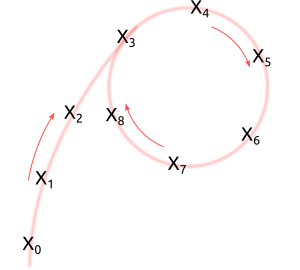
\includegraphics[width=0.6\linewidth]{pollardrho.png}
\end{center}

\subsection{Algorithme}

\begin{algorithm}[H]
\SetAlgoLined
Paramètre 1 : $n$ module de chiffrement ($n = p \times q$) \\
Paramètre 2 : $x_0$ valeur initiale pour la suite \\
\KwResult{Le facteur premier}
    $x \xleftarrow{} x_0$ \;
    $y \xleftarrow{} f(x) \bmod n$ \;
    \While{$p = 1$}{
        $x \xleftarrow{} f(x) \bmod n$ \;
        $y \xleftarrow{} f(f(y)) \bmod n$ \;
        $p \xleftarrow{} \gcd(| x - y |, n)$ \;
    }
    \eIf{$p = n$}{
        échec \;
    }{
        return $p$ \;
    }

\caption{$\rho$ pollard}
\end{algorithm}


\newpage
% ---
\section{Algorithme $p - 1$ de Pollard}

\subsection{Description}

L'algorithme $p - 1$ de Pollard vise a trouver $p$ et $q$ en ayant connaissance de $n$.
Le problème c'est que cette méthode n'est pas généraliste et ne marche qu'avec des entiers dont les facteurs possèdent une forme particulière.

\subsection{Algorithme}

\begin{algorithm}[H]
\SetAlgoLined
Paramètre 1 : $n$ module de chiffrement ($n = p \times q$) \\
Paramètre 2 : $b$ la borne maximale pour l'itération \\
\KwResult{Le facteur premier}
    $j \xleftarrow{} 2$ \;
    $a \xleftarrow{} 2$ \;
    \While{$j \le b$}{
        $a \xleftarrow{} a^j[p]$ \;
        $d \xleftarrow{} \gcd(a - 1, n)$ \;
        $j \xleftarrow{} j + 1$ \;        
    }
    \eIf{$1 < d < n$}{
        return $d$ \;
    }{
        échec \;
    }

\caption{$p - 1$ pollard}
\end{algorithm}


\newpage
% ---
\section{Méthode de factorisation de Fermat}

\subsection{Description}

Cet algorithme se base sur la décomposition de $N$ sous la forme de deux carrés $N = a^2 - b^2$. \\
Elle peut se factoriser en $(a + b)(a - b)$ à l'aide des identités remarquables.\\
Comme dans cette situation $N$ est toujours impair alors $N = 2n + 1$ et par une factorisation avec identité remarquable
$N = (n + 1)^2 + n^2$. \\ 
On a donc $a = (n + 1)$ et $b = n$.

La méthode consiste donc à trouver un $a$ tel que $a^2 - n$ soit carré et une fois que l'on a trouvé $a$, 
$b$ se déduit facilement grâce à la relation $a^2 - N = b^2$.
\subsection{Algorithme}

\begin{algorithm}[H]
\SetAlgoLined
Paramètre 1: $n$ impaire \\
\KwResult{Le couple de facteurs premiers}
    $A \xleftarrow{} \operatorname{partie\ entiere} ( \operatorname{\sqrt{n}} )$ \;
    $Bsq \xleftarrow{} A \times A - n$ \;
    \While{$Bsq$ n'est pas un carré}{
        $A \xleftarrow{} A + 1$ \;
        $Bsq \xleftarrow{} A \times A - n$ \;
    }
    return ($A - \sqrt{Bsq}$, $A + \sqrt{Bsq}$)
\caption{Fermat}
\end{algorithm}


\newpage
% ---
\section{Comparaison de temps}

Nous avons réalisé un graphe en fonction temps par rapport a la taille de n, entier représentant le module de chiffrement par rapport à une échelle logarithmique. \\
On a choisi de faire deux types de comparaisons sur chacun des algorithmes:
\begin{itemize}[label=\textbullet]
    \item Un graphe sur des petits $p < 10 000$ et $q < 10 000$, donc $n < 10^8$.
    \item Un Graphe sur n de taille 3 jusqu'a 64 bits.
\end{itemize}

\subsection{Algorithme $\rho$ (rho) de Pollard}

\begin{center}
    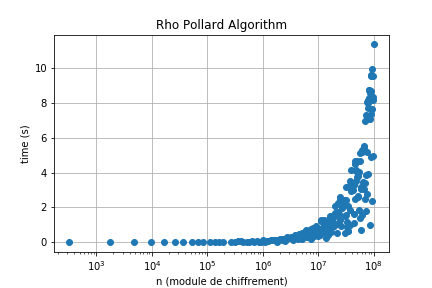
\includegraphics[width=0.7\linewidth]{images/rho_big.png}
    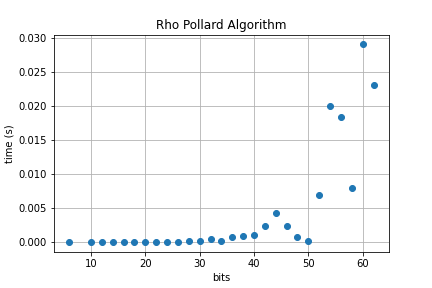
\includegraphics[width=0.7\linewidth]{images/rho_small.png}
\end{center}

\subsection{Algorithme $p - 1$ de Pollard}

\begin{center}
    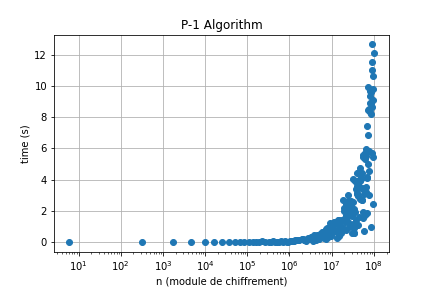
\includegraphics[width=0.7\linewidth]{images/p_one_big.png}
    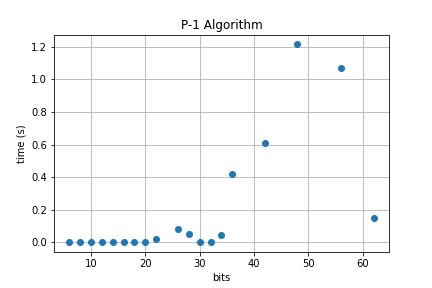
\includegraphics[width=0.7\linewidth]{images/p_one_small.png}
\end{center}

\subsection{Méthode de factorisation de Fermat}

\begin{center}
    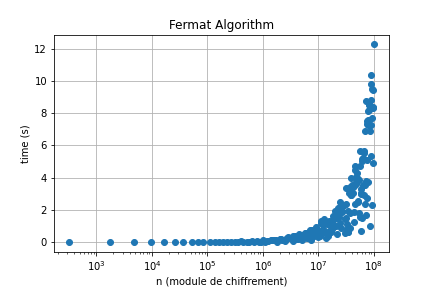
\includegraphics[width=0.7\linewidth]{images/fermat_big.png}
    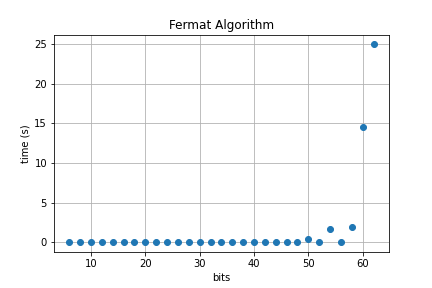
\includegraphics[width=0.7\linewidth]{images/fermat_small.png}
\end{center}

On peut voir que l'algorithme $\rho$ (rho) de Pollard est celui qui se débrouille le mieux sur des grands nombres de 64 bits :

\begin{itemize}[label=\textbullet]
    \item {Algorithme $\rho$ (rho) de Pollard} : 0,030 secondes
    \item {Algorithme $p - 1$ de Pollard} : 1,2 secondes
    \item {Méthode de factorisation de Fermat : 25 secondes}
\end{itemize}
\bigskip

Globalement pour les petits premiers les algorithmes se valent et leur temps d'exécution se ressemblent.

\end{document}
